\section{Organisation de la solution}

Le but est de trouver des algorithmes qui soient compatibles avec un grand nombre de joueurs, au delà des considérations de jouabilité au niveau du gameplay.

Le programme fourni est rédigé en Java en utilisant les bindings Java de Simgrid.
Comme le sujet est vaste, nous avons décidé d'organiser le code en plusieurs parties~: 

\begin{figure}[h!]
	\centering
	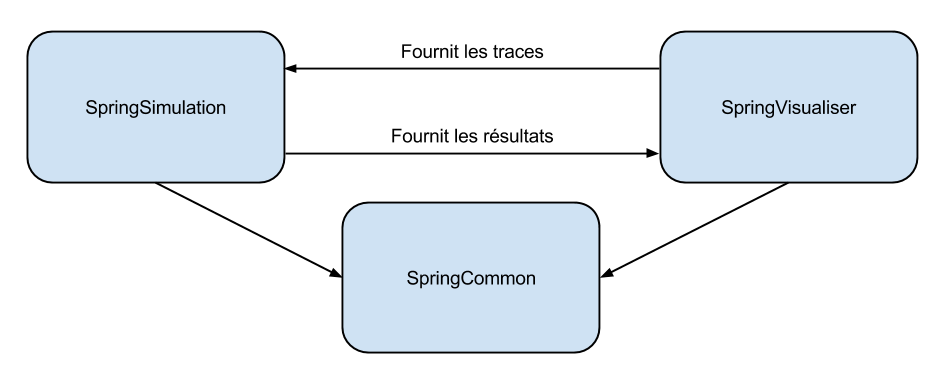
\includegraphics[width=0.8\textwidth]{orga_generale.png}
	\\[0.2cm]
	\caption{Organisation générale du code}
	\label{fig:orga}
\end{figure}

\begin{itemize}
\item SpringVisualizer~: permet de générer des traces de mouvement de joueurs, de visualiser leur déroulement et de visualiser la répartition en serveur après la simulation.
\item SpringSimulator~: le coeur de simulation, simule l'architecture réseau tout en utilisant les traces générés dans le Visualizer pour les mouvements des clients.
\item SpringCommon~: les classes en commun des deux autres projets.
\end{itemize}

\subsection{SpringVisualizer}

SpringVisualizer permet la génération des traces de mouvement de joueurs qui se fait en amont de la simulation de l'architecture de serveur.
La performance du Visualizer n'est pas primordiale car elle faite séparément et une unique fois avant la simulation des algorithmes.

\begin{figure}[h!]
	\centering
	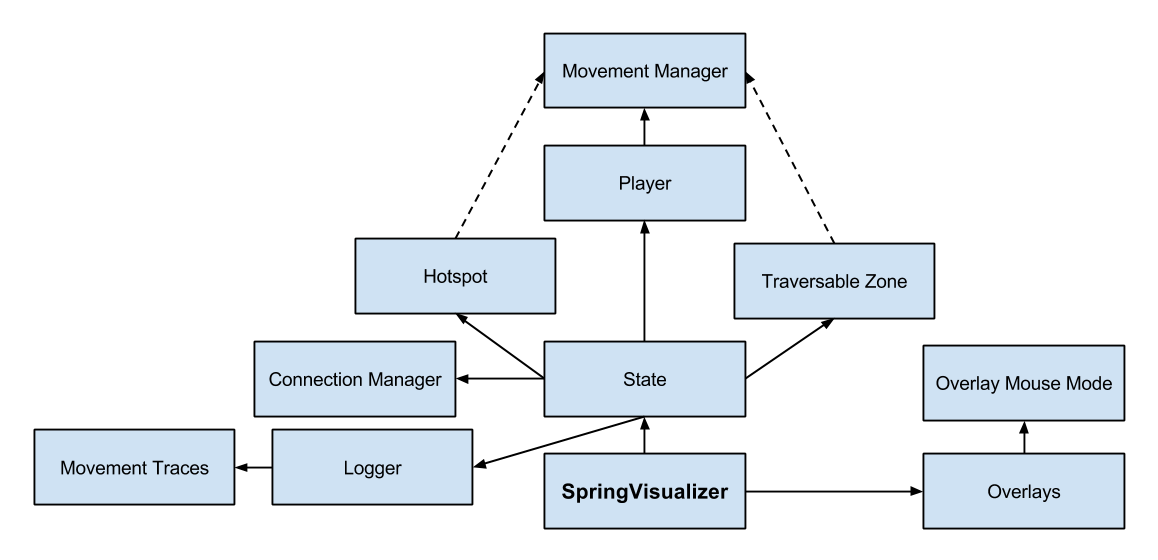
\includegraphics[width=0.8\textwidth]{SpringVisualizer.png}
	\\[0.2cm]
	\caption{Organisation du visualisateur}
	\label{fig:orga_visu}
\end{figure}

\subsubsection{Modèle}

Le programme permet de générer des traces de joueurs se déplaçant sur une carte rectangulaire.
La taille est paramétrable (sizex et sizey).
Les joueurs sont représentés à l'aide de leur identifiant et de leur position dans l'espace de jeu.
Une graine de génération permet de fixer l'aléatoire pour permettre la reproductabilité des expérimentations.
La classe Parameters réunit tout les paramètres de la génération.

\subsubsection{Interface}

Le programme dispose d'une interface graphique représentant des calques activables pour la visualisation des mouvements de joueurs~:

\begin{itemize}
\item Une image de fond pouvant représenter le monde du jeu (carte),
\item les joueurs,
\item les hotspots
\item la traversabilité des zones,
\item les zones gérées par chaque serveur,
\end{itemize}

Tout l'affichage est étiré aux dimensions de l'image de fond (si chargée) pour permettre la visualisation indépendante des coordonnées internes utilisées.
Il est possible de créer ses propres calques pour l'application.
Pour cela, il suffit d'étendre la classe \textit{AbstractOverlay} et de s'ajouter à la création de la \textit{MainWindow}.
Il est également possible de créer un nouveau mode de gestion de la souris en ajoutant à l'overlay un ou des \textit{OverlayMouseMode}.

\begin{figure}[h!]
	\centering
	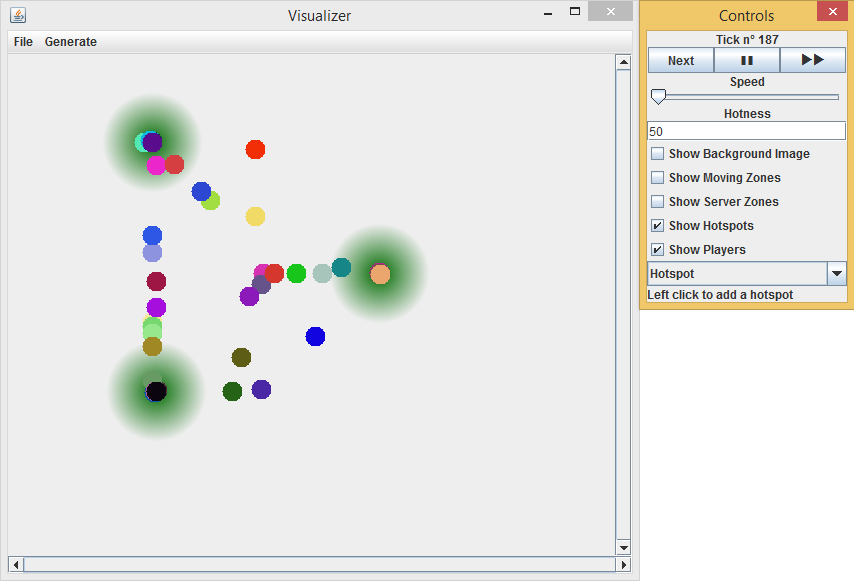
\includegraphics[width=0.8\textwidth]{capture_ecran.png}
	\\[0.2cm]
	\caption{Capture écran du visualisateur}
	\label{fig:screenshot_visualizer}
\end{figure}

\subsubsection{Modèle de mobilité}

Dans le modèle simulé, les joueurs se déplacent sur une carte rectangulaire.
Le modèle a subi plusieurs rafinement successif pour faire tendre le modèle vers plus de réalisme.

\paragraph{Mouvements Aléatoires Uniformes\\}
Tout d'abord, il a été considéré des mouvements aléatoires comme dans~\cite{interest_management_algorithm}.
Bien que cela puisse permettre de mesurer la performance des algorithmes d'\textit{Interest Management}, ce type de mouvement ne met pas en évidence de grosses variations de densité qui sont la cause des crashs du serveur de jeu.

\paragraph{Vols de Lévy\\}
Il a été observé dans les traces de Second Life~\cite{blue_banana} que les personnes se déplacent en effectuent de petits et grands déplacements alternés aléatoirement, les petits mouvements étant préférés.
Les vols de Lévy est un modèle de déplacement aléatoire qui, à chaque itération, choisis un déplacement d'une certaine distance de façon isotropique et aléatoire.
La distance de ce déplacement est définie par une fonction de distribution probabiliste.
La probabilité de faire un déplacement de taille $D$ est inversement proportionnelle à $D$.
Plus précisément, qu'un déplacement $D$ soit plus grand que $u$ est $P(D>u)=O(u^{-k})$ avec $1<k<3$.
Cela signifie que la fonction de distribution a une répartition de type puissance.

\begin{figure}[h!]
  \centering
  \caption{Exemples de 1000 pas d'un vol de Lévy en 2 dimensions, débuté en [0,0]}
  \label{fig:levy}
  \begin{subfigure}[b]{5cm}
    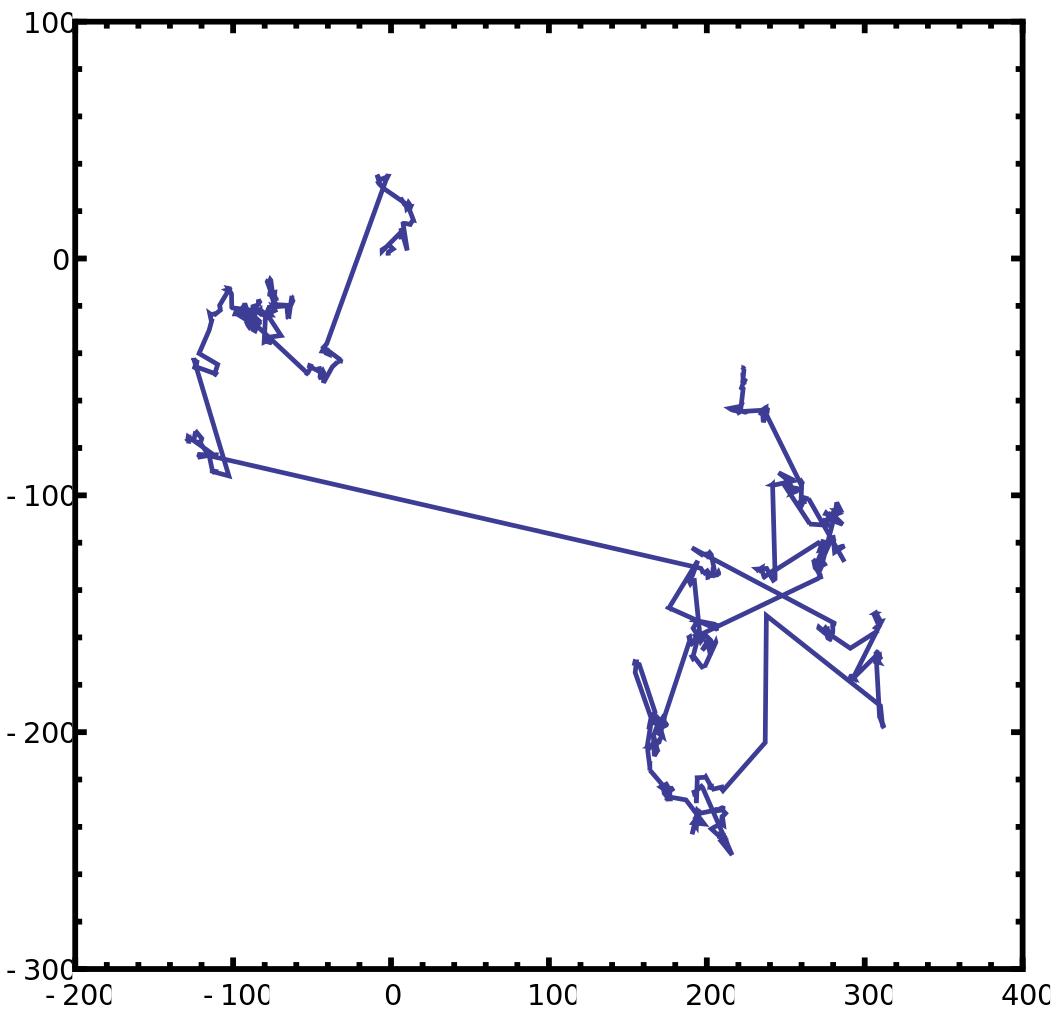
\includegraphics[width=\textwidth]{levy_1.png}
    \caption{Avec une distribution de Cauchy}
    \label{fig:levy_1}
  \end{subfigure}
  \qquad
  \begin{subfigure}[b]{5cm}
    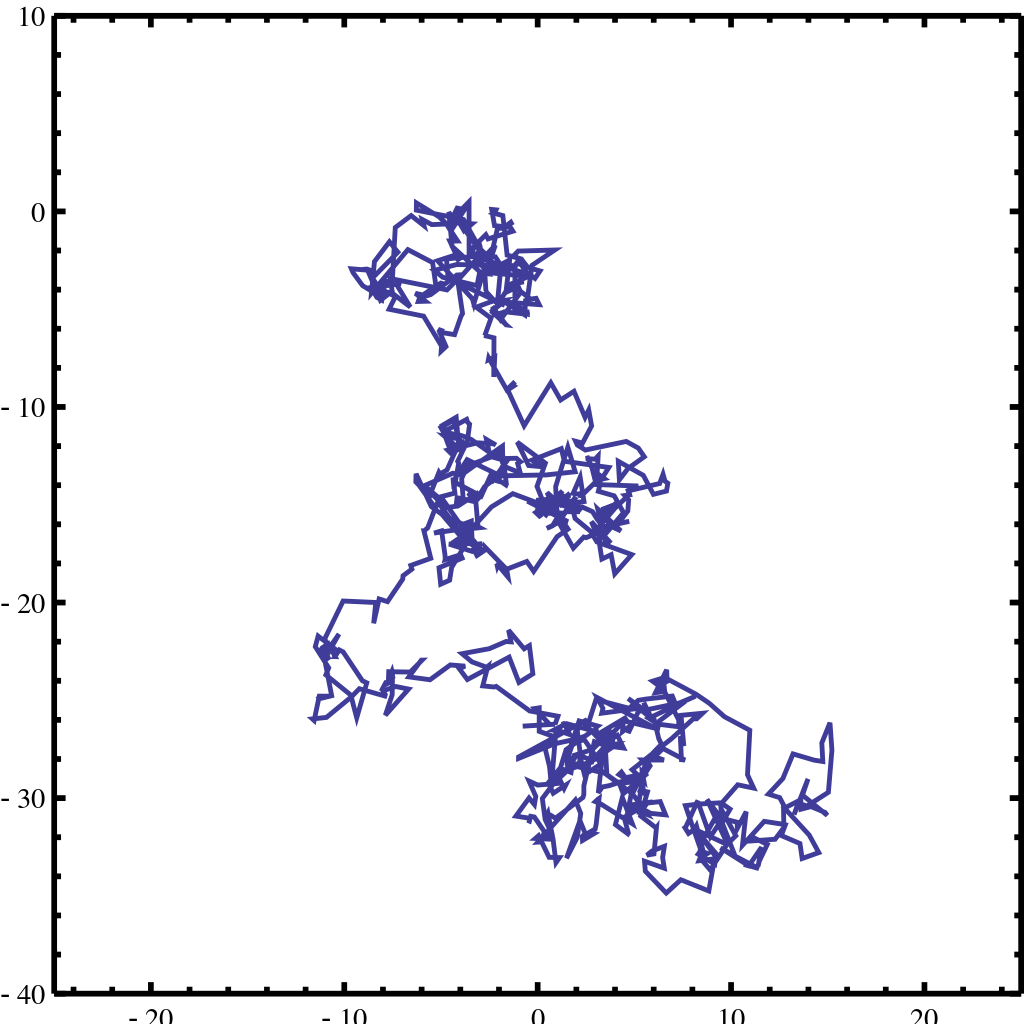
\includegraphics[width=\textwidth]{levy_2.png}
    \caption{Avec une distribution normale}
    \label{fig:levy_2}
  \end{subfigure}
\end{figure}

Le résultat de cette génération est des mouvements sur de courtes distances avec de plus rares grands mouvements entre deux points.
Cela représente les mouvements des personnes dans la vie réelle, de petits mouvements étant éffectué dans une ville et de plus rare grands mouvements effectués entre deux villes.
Les vols de Lévy modélisent également les mouvements animaliers de chasse de nourriture.
Cependant, cela ne permet pas non plus de créer des zones de densité de joueurs, bien que cela soit plus réaliste, les mouvements étant toujours aléatoires.

\paragraph{Hotspots et Blue Banana\\}
Il existe dans les jeux vidéos des zones d'intérêt qui attirent les joueurs.
Cela peut correspondre à des villes (lieux de sociabilisation) ou à des zones contenant des ressouces intéressantes pour le joueur (lieux de \textit{farm}).
Ces lieux d'attractions sont appelés \textit{Hotspots} (ou ``points chauds'') dans la littérature.
Pour effectuer une répartition correspondant à ce modèle, nous avons effectué les grands mouvements des vols de Lévy entre les Hotspots.
Cependant, cela a pour effet de bord de regrouper tout les joueurs au centre du Hotspot et donc d'entraîner un très grand gradient de densité autour des Hotspots.

\paragraph{Attirance des Hotspots\\}
Dans la réalité et dans les jeux vidéos, certains Hotspots attirent plus ou moins de personnes.
Un degré d'attirance du Hotspot, appelé \textit{hotness}, a donc été ajouté et corresponds à une probabilité d'aller vers ce Hotspot.
Cela entraîne donc des variations dans la concentration de joueurs autour des Hotspots en fonction de leur intérêt, ainsi que la mise en place d'attirance temporaire en faisant varier l'attractivité des Hotspots.

\paragraph{Répartition des joueurs autour des Hotspots\\}
Il a été observé que la répartition des joueurs autour des Hotspots suit une loi de puissance~\cite{these_raluca}.
Cela entraine une très grande concentration au centre du Hotspot qui devient plus diffuse plus on s'éloigne du centre.
Cependant, les vols de Lévy seuls ne permettent pas d'effectuer ce type de concentration.
Un rayon de répartition a donc été ajouté autour des Hotspot afin de permettre d'avoir des répartitions plus ou moins grande en fonction de la taille du centre d'intérêt.

\begin{figure}[h!]
	\centering
	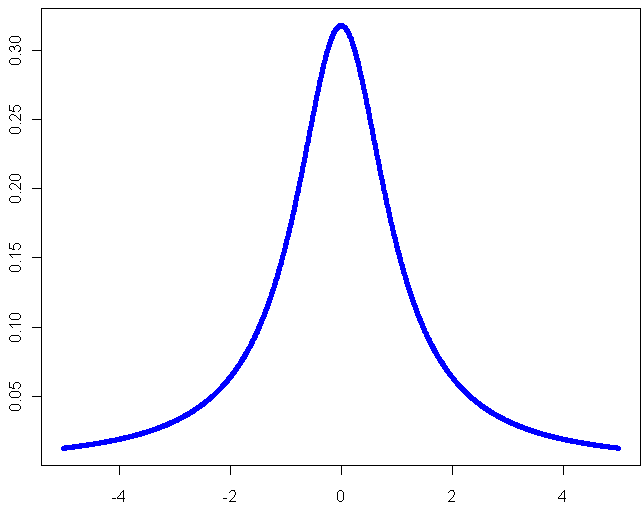
\includegraphics[width=0.5\textwidth]{cauchy.png}
	\\[0.2cm]
	\caption{Probabilité de répartition autour d'un hotspot en fonction de la distance par rapport au centre.}
	\label{fig:repartition}
\end{figure}

\paragraph{Nombre de joueurs\\}

Le nombre de joueurs évolue au cours du temps comme indiqué dans la partie II.1.
Pour modéliser ce phénomène, nous avons donc généré des connexions et déconnexions de joueurs en suivant une fonction décrivant le nombre de joueurs à chaque tick.
Notre modèle comprends~:

\begin{itemize}
\item Une croissance de type exponentielle au début pour représenter le pic de connexion au lancement du MMOG.
\item Une variation sinusoïdale pour représenter la connexion diurne des joueurs.
\item Des croissances et décroissances linéaires couplées à la sinusoïdale pour indiquer le gain ou la perte en popularité du jeu au cours du temps et mettre en évidence le phénomène de saturation et libération des serveurs.
\end{itemize}

Notre but étant de mettre en évidence le phénomène de saturation de l'architecture de serveurs, il faudra donc qu'il y ait plus de phases de croissance que de décroissance.

\begin{figure}[h!]
	\centering
	\framebox{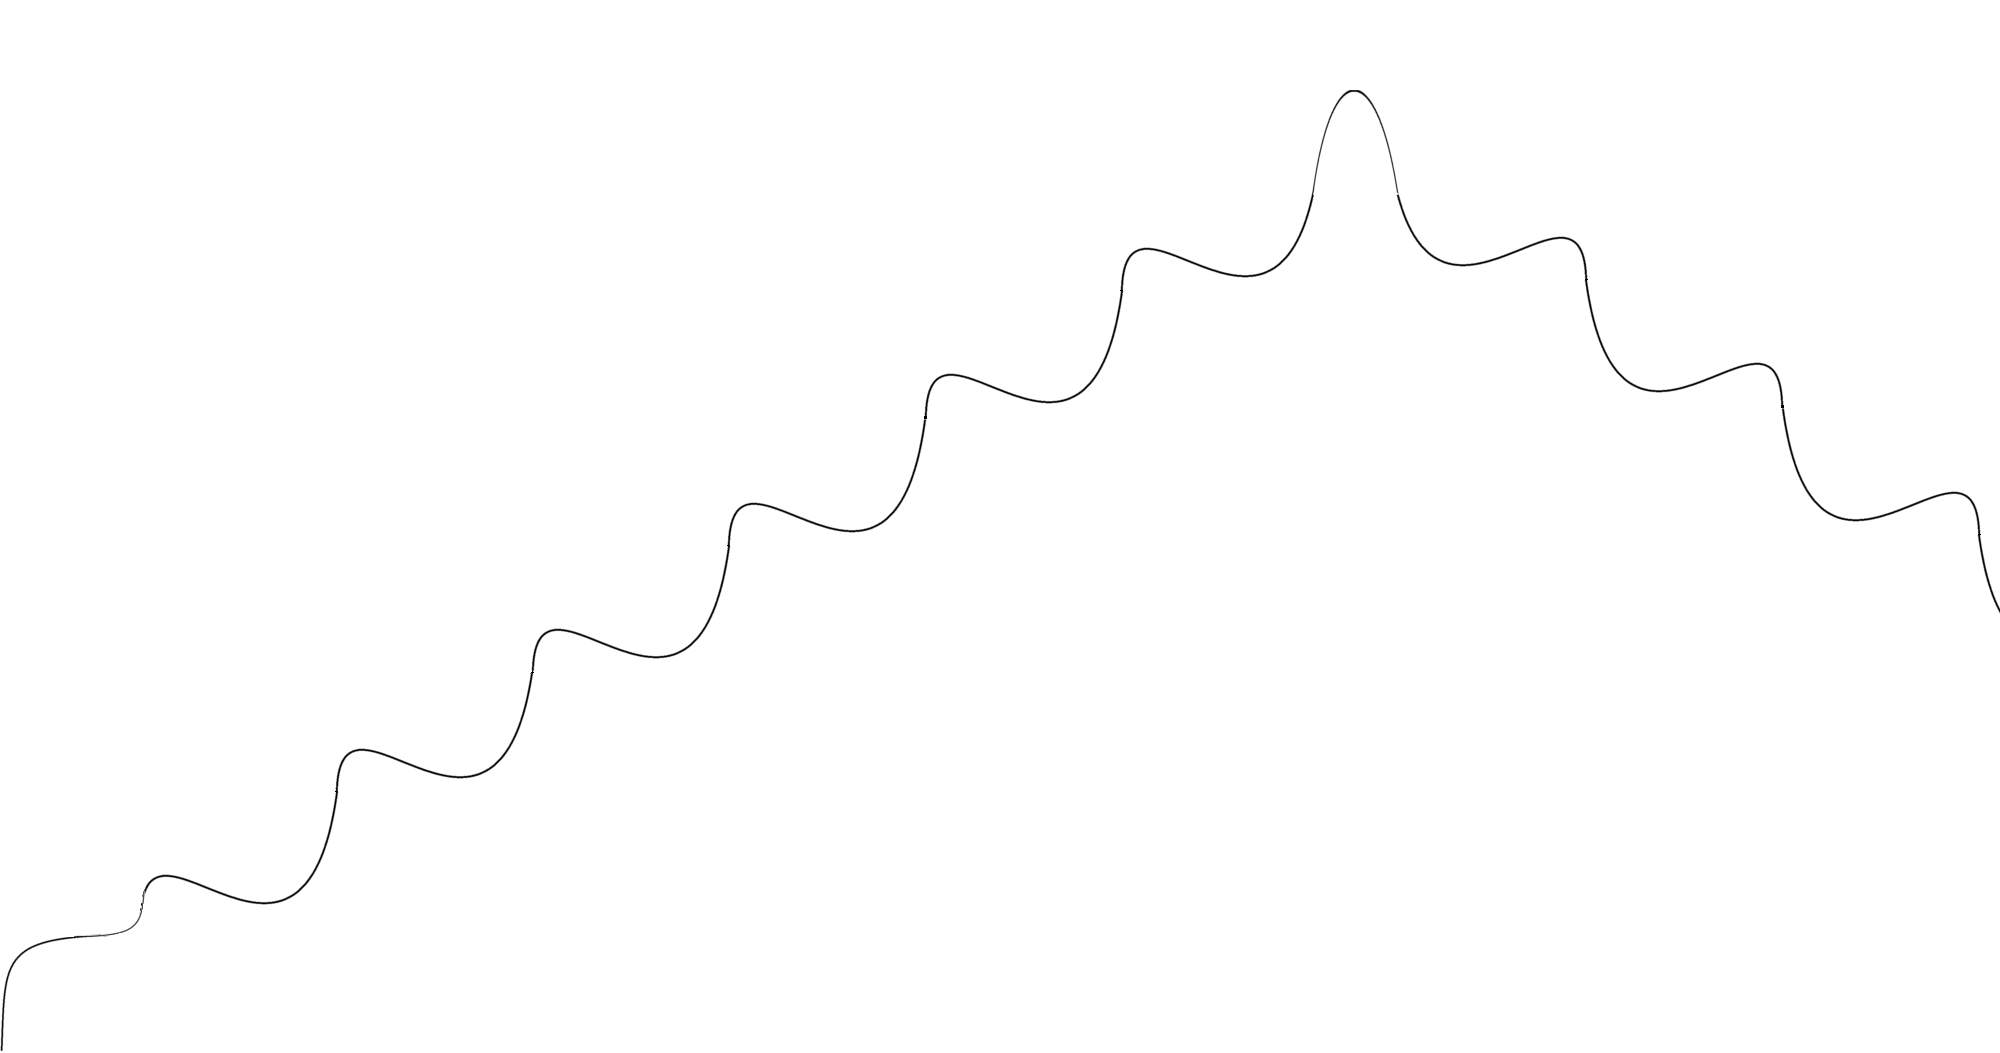
\includegraphics[width=0.5\textwidth]{nbre_joueurs.png}}
	\\[0.2cm]
	\caption{Evolution du nombre de joueurs en fonction du temps.}
	\label{fig:nbre_joueurs}
\end{figure}

\paragraph{Traversabilité de zones\\}
La majeure partie du temps, une zone de jeu n'est pas intégralement accessible.
Il existe par exemple du relief ou des océans qui peuvent entraver les mouvements du joueur et entraîne des zones interdites.
Cela oblige les joueurs à contourner ces obstacles et crée donc des zones de passage, par exemple une vallée entre deux chaînes de montagnes.
Dans le programme, nous avons donc permis de choisir quelles sont les zones accessibles par les joueurs avant la génération des traces.
La traversibilité des zones est stockée dans un QuadTree pour permettre une précision modulable en fonction de la zone.

\begin{figure}[h!]
	\centering
	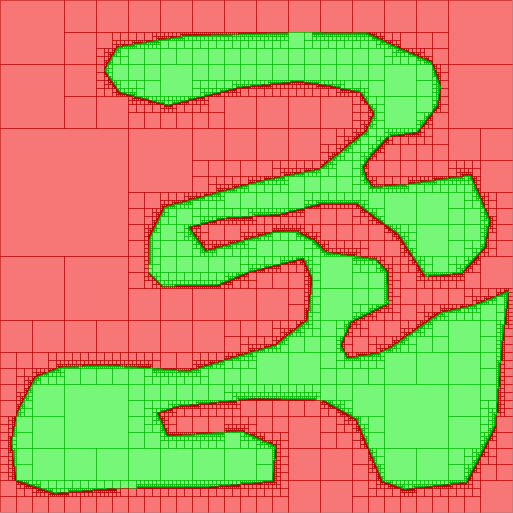
\includegraphics[width=0.5\textwidth]{zones.png}
	\\[0.2cm]
	\caption{Exemple de zones et de leur stockage en QuadTree. Le rouge indique les zones infranchissable.}
	\label{fig:zones}
\end{figure}

La création de ces zones non traversables entraîne donc un problème dans la génération des mouvements, les mouvements ne pouvant plus s'effectuer en ligne droite entre les hotspots ou n'importe où sur la carte pour les déplacements à l'intérieur d'un hotspot.
Il faut donc utiliser du pathfinding sur la carte en utilisant le QuadTree pour les zones inaccessibles.

\subsubsection{Pathfinding}

La recherche d'un plus court chemin dans le QuadTree entre un point de départ et d'arrivé correspond à la recherche d'un plus court chemin dans un graphe.
Ce graphe possède des poids sur les arrêtes qui seront nommées par la suite $c_{p-q}$, le poids de l'arrête entre les sommets $p$ et $q$.

\paragraph{Dijkstra\\}
Pour la recherche de plus court chemin dans un graphe, la solution usuelle est d'utiliser l'algorithme de Dijkstra qui est un algorithme simple à implémenter.
Dans cet algorithme, on utilise un liste $l$ on affecte un poids $d_{noeud}$ à chaque noeuds du graphe, initialisé à l'infini au départ, et un noeud de provenance $a_{noeud}$.
La point de départ est initialisé à 0 sans noeud de provenance et est ajouté à la liste $l$.
Tant que le point d'arrivée n'est pas trouvé, on prends le noeud $p$ de $l$ ayant le poids le plus faible.
Pour chacun des noeuds $q$ atteignable à partir de ce noeud $p$, si $d_{p} + c_{p-q} < d_{q}$, alors $d_{q} = d_{p} + c_{p-q}$, $a_{q} = p$ et le noeud est ajouté à $l$.
Lorsque le noeud d'arrivée à été atteint, il suffit de suivre le chemin formé par les antécédents pour obtenir le chemin le plus court.

Le problème de cet algorithme est qu'il explore de nombreux points et dans toute les directions car il ne prends prends pas en compte si le point est dans la direction du point d'arrivée.
L'idée de l'algorithme A* est donc de prendre en compte un estimation de la distance restante avec l'objectif pour chacun des points.

\paragraph{A*\\}
Pour permettre un pathfinding efficace, nous nous sommes tournés vers la solution couramment implémentée dans le domaine de l'intelligence artificielle qui est l'A*.
Celui-ci est plus rapide que l'algorithme de Dijkstra mais ne donne pas forcément le meilleur chemin.
Il garantit cependant que le premier chemin trouvé par l'algorithme est un des meilleurs chemin.
L'exactitude du meilleur chemin n'est pas important dans notre solution car le déplacement que nous souhaitons avoir doit simuler un mouvement humain qui n'est pas forcément optimal.

Le fonctionnement est le même que Dijkstra, sauf que le poids de chaque noeud $p$ est déterminé par $f(p) = g(p) + h(p)$, avec $g$ le coût de la distance déjà parcourue, comme le coût dans l'algorithme de Dijkstra, et $h$ la fonction d'heuristique.
Cette fonction d'heuristique est une fonction d'estimation du coût du chemin restant.
On peut remarquer que Dijkstra est un cas particulier de A* où $h(x) = 0$ pour tout x.
Un exemple de fonction d'heuristique est la distance de Manhattan~: pour $A(X_{A}, Y_{A})$ et $B(X_{B}, Y_{B})$, $d(A, B) = |X_{B} - X_{A}| + |Y_{B} - Y_{A}|$.

Cependant, bien que A* soit rapide pour trouver un chemin, celui-ci peine lors des grands chemins avec de nombreux murs dù à l'exploration de nombreux noeuds, à une liste de points à explorer très grande et un coût de calcul de la fonction d'heuristique qui peut être important.

\paragraph{A* + Jump Point Search (JPS)\\}
JPS~\cite{jps_article} est une amélioration de l'algorithme A* dans les grilles à coût uniforme (ce qui est le cas ici, le coût étant la distance parcourue).
Il exploite l'équivalence des chemins vis-à-vis de la symétrie.

\begin{figure}[h!]
	\centering
	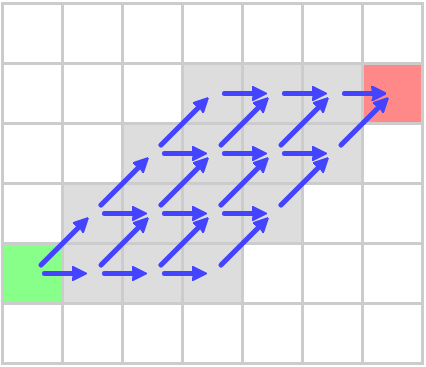
\includegraphics[width=0.4\textwidth]{symetrie_JPS.png}
	\\[0.2cm]
	\caption{Illustration de l'équivalence des chemins symétriques}
	\label{fig:symetrie_JPS}
\end{figure}

Pour explorer l'intégralité du graphe, JPS utilise une exploration verticale et horizontale suivie d'une exploration diagonale.
Lors d'un déplacement horizontal ou vertical (voir \textsc{Figure}~\ref{fig:explo_jps}), provenant de 4 et arrivant à x, il est inutile de s'intéresser aux voisins $\{2, 3, 7, 8\}$ car ceux-ci seront explorés par parcours diagonal puis horizontal ($\overrightarrow{42} + \overrightarrow{23}$), dont le coût est moins élevé à cause de la diagonale.
De même, lors d'un parcours diagonal, il est inutile de considérer les voisins $\{1, 4, 7, 8\}$ car ceux-ci ont déjà été exploré par parcours vertical et horizontal.

\begin{figure}[h!]
	\centering
	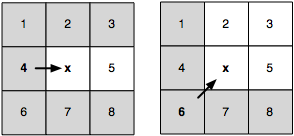
\includegraphics[width=0.5\textwidth]{explo_jps.png}
	\\[0.2cm]
	\caption{Exploration du graphe à l'aide de JPS}
	\label{fig:explo_jps}
\end{figure}

Cependant, si il y a un endroit inaccessible suivi d'un endroit accessible dans les voisins ingnorés plus haut, comme le montre la \textsc{Figure}~\ref{fig:jmp_point_jps}, il est nécessaire d'effectuer un parcours à partir de ce point car il y a des points qui ne seront pas explorés par d'autres itérations du parcours (les points entourés en rouge).
Ces points-ci, ainsi que le point d'arrivée, sont appelés Jump Points et sont ceux ajoutés à la liste de points à explorer.
Il est donc inutile de calculer $f(p)$ pour chacun des points mais uniquement pour ces Jump Points.
Bien que plus de points ne soient explorés que dans A*, le temps de calcul pour chacun des points est beaucoup plus faible.

\begin{figure}[h!]
	\centering
	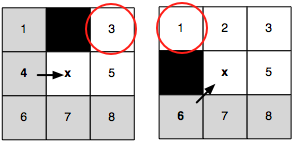
\includegraphics[width=0.5\textwidth]{jmp_point_jps.png}
	\\[0.2cm]
	\caption{Jump Points de l'algorithme JPS}
	\label{fig:jmp_point_jps}
\end{figure}

\paragraph{Améliorations\\}

Diverses amélioration au niveau du code ont été nécessaire pour obtenir une vitesse convenable d'exécution de l'algorithme par rapport à une implémentation directe.

Tout d'abord, au niveau de la liste des points à explorer, il est nécessaire d'obtenir le noeud ayant le poids le plus faible.
Utiliser une simple liste où les éléments sont non triés entraîne une insertion en $O(1)$ mais une récupération de l'élément le plus faible en $O(n)$, avec n le nombre d'éléments dans la liste.
A l'aide d'une liste triée, il est possible d'insérer les éléments avec une complexité en $O(\log(n))$ en cherchant l'emplacement d'insertion de façon dichotomique mais de récupérer l'élément de poids le plus faible en $O(1)$.
Cependant, il a été observé à l'aide d'un profiler que cette méthode s'est révélé très lente.
Ceci est dù à la manière dont est effectuée l'opération de suppression et de récupération d'un élément dans la liste (opération \textit{remove(int)}).
Celle-ci, lorsque appliquée au premier élément, récupère cet élément et décale l'intégralité du tableau de stockage interne d'une case vers la gauche, qui est une opération en $O(n)$.
Pour permettre d'utiliser une liste triée de cette manière, il a donc fallu trier par ordre décroissant et retirer le dernier élément plutôt que le premier, ce qui entraîne un très grand gain de performance.

La seconde optimisation est au niveau de l'identifiant d'un noeud dans l'algorithme qui était un objet de type \textit{Point}, contenant les deux coordonnées x et y.
Cependant, l'utilisation d'une telle classe dans le code entraînait la création de nombreux objets de ce type lors du déroulement de l'algorithme.
Le temps de création de ces variables devenait donc non négligeable dans l'exécution du code.
A l'aide de l'isomorphisme $f$ écrit ci-dessous, il a été possible de remplacer les objets par des types primitifs (int), ce qui permet une optimisation en mémoire et temps de calcul.

\centering
$\begin{array}{ccccc}
f & : & \intervalle{[}{0}{size_{x}}{[}*\intervalle{[}{0}{size_{y}}{[} & \to & \intervalle{[}{0}{size_{x}*size_{y}}{[}\\
  & & \mathopen{(}x,y\mathclose{)} & \mapsto & x*size_{y}+y \\
  & & & \\ % empty line
f^{-1} & : & \intervalle{[}{0}{size_{x}*size_{y}}{[} & \to & \intervalle{[}{0}{size_{x}}{[}*\intervalle{[}{0}{size_{y}}{[} \\
 & & x & \mapsto & \mathopen{(}E\mathopen{(}\frac{x}{size_{y}}\mathclose{)},x\bmod{size_{y}}\mathclose{)} \\
\end{array}$

\justifying
Enfin, nous avons utilisé des tableaux de tailles fixes plutôt que des collections de type Map pour stocker les valeurs de poids pour chacun des noeuds explorés, en utilisant leur identifiant entier comme indice dans le tableau.
Cela évite de rechercher à chaque fois la valeur désirée dans la collection en donnant un accès en lecture et écriture en $O(1)$.

\subsection{SpringSimulator}

\begin{figure}[h!]
	\centering
	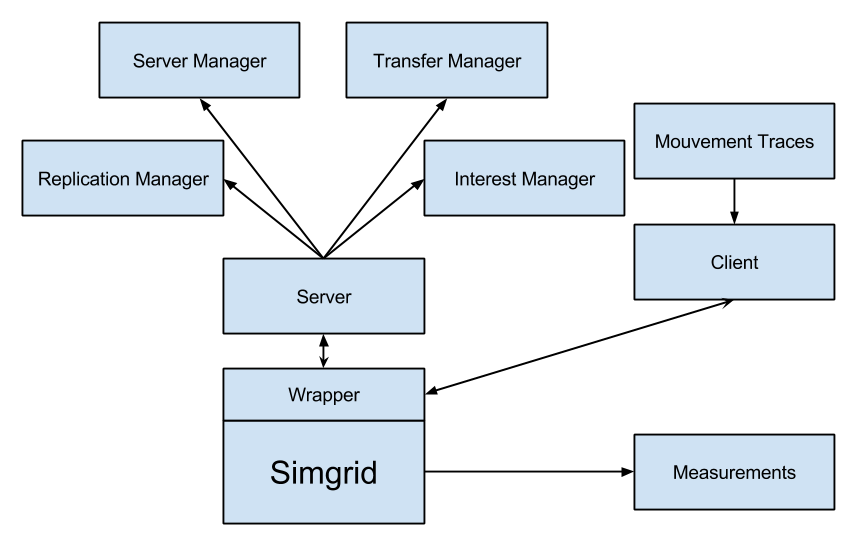
\includegraphics[width=0.8\textwidth]{SpringSimulator.png}
	\\[0.2cm]
	\caption{Organisation du simulateur}
	\label{fig:orga_simu}
\end{figure}

Notre but pour le simulateur est d'avoir une plateforme suffisamment générique pour étudier différent types d'architectures.
Celui-ci adopte un modèle simple, basé sur le \textit{Zoning}.
Les serveurs gèrent des zones $Z$ telles que:

\centering
$\begin{array}{cc}
\forall\,\mathopen{(}i,j\mathclose{)}\in \llbracket 1,nbserv \rrbracket ^{2},\quad i \neq j \;\Rightarrow\; Z_{i} \cap Z_{j} = \varnothing \vspace{2mm}\\
et\vspace{1mm}&\\
\bigcup\limits_{i=1}^{nbserv} Z_{i} = \Omega
\end{array}$

\justifying
C'est a dire que les zones $Z$ gérées par les serveur forment une partition de l'univers du jeu vidéo.
Chaque serveur est responsable des joueurs situé dans leur zone.

\subsubsection{Modèle}

Nous avons choisis d'utiliser une organisation des machines pour le cloud permettant de régler plusieurs paramètres.
Tous les clients, ayant leur propre connexion internet (Download, Upload et Latence) sont reliés à un seul et même routeur (``Internet'') car la connexion internet des clients n'ont pas d'influence sur celle des autres.
Les serveurs sont tous reliés à un autre routeur (``Gateway'') qui correspond à la connexion internet de l'architecture de serveurs.
Le réseau local à l'intérieur de l'architecture de serveurs est rapide et permet l'échange de données rapide entre les serveurs.
SpringVisualizer permet de générer un fichier de plateforme correspondant à cette organisation.
Le fichier de plateforme de Simgrid correspond à l'organisation des machines (\textit{Host}) et leurs liens réseaux avec leur latences (\textit{Link} et \textit{Route}).
Pour gérer un nombre dynamique de serveur, un nombre maximum est défini en amont et les machines ne sont pas directement incluses dans l'architecture de serveur.

Un wrapper de Simgrid a été mis en place pour isoler la partie simulation des algorithmes.
Cela permettra à terme de passer de la simulation à un prototype plus simplement.
Les algorithmes utilisés dans la simulation sont séparés en plusieurs modules distincts.

\paragraph{Interest Management\\}
Cette partie du serveur correspond à la zone d'intérêt du joueur, c'est à dire de savoir quelles sont les données pertinentes à envoyer à un joueur lors de mise a jour de l'état du monde de jeu.
Les actions dans un jeu vidéo étant la plupart du temps locales avec un effet local, la zone d'intérêt d'un joueur se trouve souvent être un cercle centré autour du joueur.

De nombreux algorithmes pour résoudre ce problème existent déjà~\cite{interest_management_algorithm}.
Cependant, il faudra vérifier lequel est le plus efficace dans cette architecture de serveur pour minimiser les calculs ainsi que les transferts entre serveurs tout en gardant une vue correcte pour le client.

Une solution possible est d'utiliser un rayon constant autour du joueur correspondant au champ de vision du joueur.
Cependant, en cas de zone surchargée, de nombreuses données lui sont envoyés, ce qui ralentit l'envoi des nouveaux états et l'affichage du client.
Une solution est donc d'adjoindre une notion de densité qui ne permet d'envoyer qu'un certain rayon plus petit.

\paragraph{Replication Management\\}
Cette entité permet de répliquer des zones entre les serveurs.
Chaque donnée possède un serveur responsable, qui transmet les mises à jour aux réplicats.
Cela permet en cas de crash de ne pas perdre les données car celles-ci sont aussi stockées dans la mémoire d'autres VM.
En supposant les crashs isolés et indépendants (les VM étant réparties convenablement pour éviter une déconnexion totale de l'architecture), il suffit de répliquer les zones au moins une fois pour ne pas perdre de données.

De plus, en réplicant les zones frontalières entre serveurs cela permet d'avoir des données d'un autre serveur pour éviter les requêtage à chaque tick pour l'envoi du nouvel état du monde.
Pour faire ceci efficacement, il faut prendre en compte les zones d'intérêt définies par les algorithmes d'\textit{Interest Management}.
Cela permet de faire des transferts de joueurs entre serveurs aux frontières de manière plus douce, en ne changeant que le responsable au franchissement de la frontière, celui-ci étant déjà répliqué dans la zone d'overlap.

\paragraph{Transfer Management\\}
Le \textit{Tranfer Management} correspond à la gestion des transferts de zones entre les serveurs pour permettre de faire de l'équilibrage de charge, ainsi que le transfert entre serveur des clients changeant de zone.
Celui-ci prends en compte les zones déjà répliquées dans \textit{Replication Management} pour permettre une gestion efficace des transferts.
Pour permettre le transfert d'une zone, les données sont transférées au nouveau serveur ainsi que les opérations en attente de traitement sur cette zone.
Il peut être nécessaire de garder un historique des derniers transferts pour éviter de tranférer plusieurs fois entre les deux même serveurs la même zone.

\paragraph{Server Management\\}
Le module \textit{Server Management} détermine si il est nécessaire d'allouer ou de retirer des VM dans l'architecture.
Il prends en compte l'encombrement de tout les serveurs et ajoute ou retire des VM à un endroit particulier pour libérer de la charge ou des marchines.

Plusieures stratégies peuvent être mises en places pour permettre cette allocation dynamique.
La plus simple est un système de seuillage.
Lorsque la charge d'une VM dépasse un certain seuil (par exemple 70\%) , une nouvelle VM est allouée et la charge est partagée en deux.
Lorsque la charge de deux VM voisines est en dessous d'un certain seuil (par exemple 30\%), les deux VM sont fusionnées pour libérer une machine.

Une autre méthode est d'utiliser conjointement un algorithme de learning qui peut apprendre si le pic de charge est temporaire ou nécessite l'allocation d'une autre VM.
Cela permet également de prévoir les pics habituels de joueurs aux heures de connexion et déconnexion.

\subsubsection{Métriques}

\paragraph{Latence input-résultat\\}
Un entier représentant numéro d'identification de message (un entier incrémenté à chaque message envoyé) est envoyé avec les messages.
Lorsque le serveur traite le message, il envoit avec le nouvel état du monde le numéro d'identification du dernier message traité.
Le client reçoit ainsi le nouvel état et sait que son message a été traité.
La latence prise en compte est donc $t_{reception} - t_{envoi}$, calculée côté client.

\paragraph{Tickrate\\}
Celui-ci est fixé en début de simulation.
Si les serveurs n'arrivent pas à suivre la charge des messages reçus à traiter durant un tick, des messages ne seront traités qu'au tick suivant et cet évènement est loggé dans l'application.

\paragraph{Utilisation Processeur\\}
L'utilisation du processeur (en \%) corresponds au temps de traitement des messages reçus divisé par le temps total du tick.

\paragraph{Utilisation Mémoire\\}
L'utilisation mémoire d'un serveur correspond au nombre d'objets stockés sur le serveur.
Cette métrique vaut donc le nombre de joueurs connectés et/ou répliqués par ce serveur, multiplié par la taille de stockage d'un joueur.

\paragraph{Utilisation Réseau\\}
L'utilisation réseau correspond à la bande passante utilisée sur la bande passante totale disponible, en téléchargement et envoi.
Cette métrique est mesurée à la fois chez le client et les serveurs grâce à Simgrid.

\paragraph{Prix\\}
Le prix de l'architecture dans le Cloud est un modèle qui est importé des plateformes de Cloud telles que Google Cloud~\cite{google_cloud} et Amazon EC2~\cite{amazon_ec2}.
Celui-ci dépend du type de serveur, du temps de serveur utilisé ainsi que l'utilisation de la bande passante.

\subsubsection{Tests}

Comme le stage s'est principalement orienté sur la création du modèle de mobilité réaliste et d'un outil générateur de traces suivant ce modèle, le développement des algorithmes a été repoussé au sujet de thèse.
Les tests d'algorithmes n'ont donc pas pu être effectués.
Cependant, pour s'assurer du fonctionnement de la plateforme de simulation, des scénariaux simples ont été testés avec un nombre fixe de serveurs.
Ceux-ci mettent donc en évidence des phénomènes

\paragraph{Scénario 1\\}
Le scénario utilise un nombre fixe de serveur à la séparation fixe et montre qu'un serveur n'arrive plus à suivre lors d'un pic de charge.
Deux hotspots A et B sont gérés par deux serveurs qui correspondent à deux villes.
Un troisième serveur (C) gère le reste du monde.
Les deux populations se déclarent soudainement la guerre et combattent dans la zone C.

\begin{figure}[h!]
	\centering
	\framebox{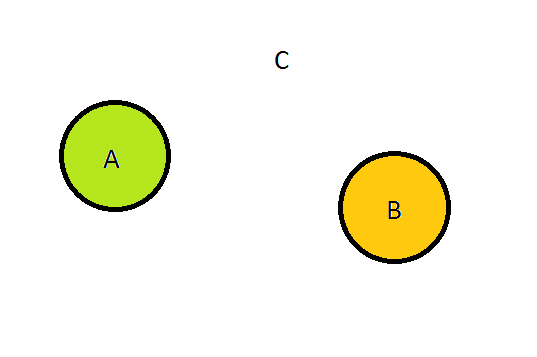
\includegraphics[width=0.5\textwidth]{scenario_1.png}}
	\\[0.2cm]
	\caption{Carte du premier scénario}
	\label{fig:scenario_1}
\end{figure}

Ce premier scénario met en évidence qu'une répartition fixe peut être valable à un certain moment mais, à cause du mouvement des joueurs, ne plus l'être dans le futur.
On observe comme escompté dans la simulation la saturation du CPU du serveur C qui n'arrive plus à gérer les demandes de mouvements des joueurs lorsqu'un certain nombre s'est réunis autour du même hotspot.

\paragraph{Scénario 2\\}
Le scénario 2 met en place deux serveurs ayant une séparation dynamique du monde.
Une zone d'overlap entre les serveurs est mis en place.
L'actualisation de cette séparation en zone s'effectue tout les X tick et tend à séparer équitablement les joueurs entre les deux serveurs.
Au bout d'un temps Y, il ne reste qu'un seul hotspot et la majeure partie des joueurs se réunissent autour.

\begin{figure}[h!]
	\centering
	\framebox{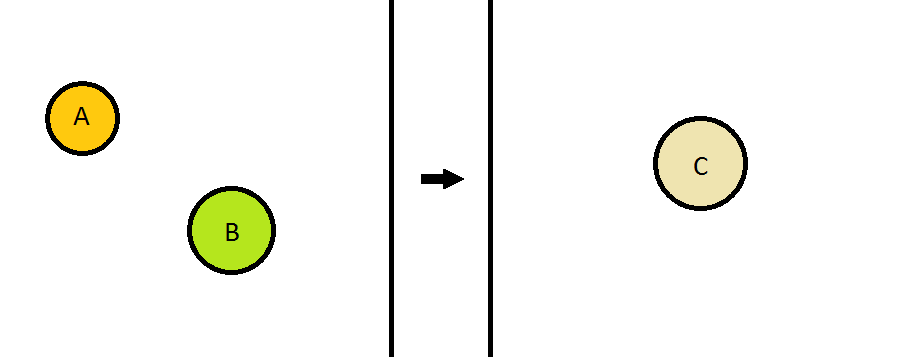
\includegraphics[width=0.5\textwidth]{scenario_2.png}}
	\\[0.2cm]
	\caption{Carte du deuxième scénario}
	\label{fig:scenario_2}
\end{figure}

Ce scénario met donc en évidence que la mise en place d'overlap va tendre à mettre un serveur responsable de la moitié des joueurs et avoir l'autre moitié en réplication.
Cela fait donc beaucoup d'échange de données à la frontière entre les serveurs.
Le réseau se trouve donc saturé et l'architecture ne peut plus répondre.
La simulation met en évidence une saturation du réseau interne à l'architecture de serveurs.

\section{Travaux futurs}

\subsection{Modèle de mobilité}

Le modèle de mobilité implémenté actuellement, bien que relativement réaliste, pourrait être raffiné.

Tout d'abord, un modèle ayant des coûts de déplacement non uniformes pourra être mis en place pour plus de réalisme.
En effet, une zone escarpée et dangereuse sera plus compliquée (et donc moins rapide) à traverser qu'une route sécurisée prévue à cet effet.
Le voyage par les routes doit donc être préféré (dans une certaine limite) au voyage le plus court actuellement effectué.
Les lois de la réfraction en optique (lois de Descartes) peuvent être utilisées pour déterminer le chemin le plus optimisé, le problème étant similaire.
Il faut également remarquer que de nombreux jeux possèdant une grande carte du monde ont tendance à proposer des ``voyages rapides'' (\textit{fast travel}) qui correspondent à des téléporteurs pour éviter les voyages répétitifs et rébarbatifs aux joueurs.

Ensuite, des mouvements de groupes pourront être proposés.
En effet, la sociabilisation est une part importante des jeux en ligne et cela entraîne donc la formation de groupes voyageant ensemble.
Pour l'architecture de serveur, cela peut se traduire par un transfert d'un très grand nombre de joueurs en même temps à un serveur voisin, ce qui peut mettre en évidence de grandes latences.

Dans la réalité, les déplacements des joueurs ne sont pas optimisés.
Il est possible d'introduire des déplacements plus ``arrondis'' pour contourner des obstacles par exemple.
Cela ajouterait à la crédibilité de la simulation de mouvement ressemblant à des mouvements humains.

Enfin, il peut être intéressant d'introduire de la dynamicité dans les zones interdites aux déplacement.
En effet, suite à certaines actions des joueurs, l'accessibilité d'une zone peut être différente.
Cela permet également de modéliser des effets de contournement de groupes pour, par exemple, permettre à des personnes étrangères à un affrontement de le contourner pour éviter des dégâts collatéraux.

\subsection{Architecture}

Comme dit dans la partie sur la simulation, une phase de learning sur les habitudes des joueurs et de l'heure pourrait permettre d'allouer à l'avance de nouvelles VM en évitant de se trouver dans une situation de surcharge durant l'apparition des nouvelles VM.
L'apparition d'une VM et le transfert de la zone dont elle sera responsable prend du temps qui peut, bien qu'ayant peut-être été activée avant la surcharge avec un seuil, durer trop longtemps pour permettre de resister le pic de charge induis.
Prévoir ce genre de comportement du système est donc intéressant pour prendre des dispositions en amont.

Pour décharger l'architecture de serveur (VM dans le Cloud), il pourrait être intéressant de se pencher sur une architecture de type hybride.
Une partie des calculs serait effectuées par les clients en utilisant un modèle de type Pair-à-Pair.
Cela peut être utilisé principalement pour des tâches n'ayant pas ou peu d'incidence dans l'expérience de jeu si les performances sont moindres.
Par exemple, la discussion instantanée à l'intérieur du jeu n'a pas autant d'importance que les mises à jour du monde de jeu, les messages pouvant arriver un peu plus tard sans trop de conséquences.

La tolérance aux fautes est quelque chose d'important pour la disponibilité de l'architecture de serveurs.
Celle-ci est partiellement assurée par la disponibilité des données grâce à la réplication car les crashs sont isolés et indépendants (sauf en cas de panne totale du fournisseur de machine virtuelle, mais rien ne peut être fait pour contrer cela).
Il suffit donc de redémarrer une autre VM en cas de crash et lui retransférer la copie des données dont la VM crashée était responsable.
Cependant, la tolérance aux fautes byzantines est beaucoup plus complexe.
Cette importance de la tolérance aux fautes byzantines est encore plus importante si il y a une utilisation d'une architecture Pair-à-Pair chez les clients.

Le but final de la thèse est de déterminer quels sont les meilleurs algorithmes et heuristiques en simulation puis de les tester en développant un prototype.
